\section{Activity Structure}

\begin{figure}[h!]
	\centering
	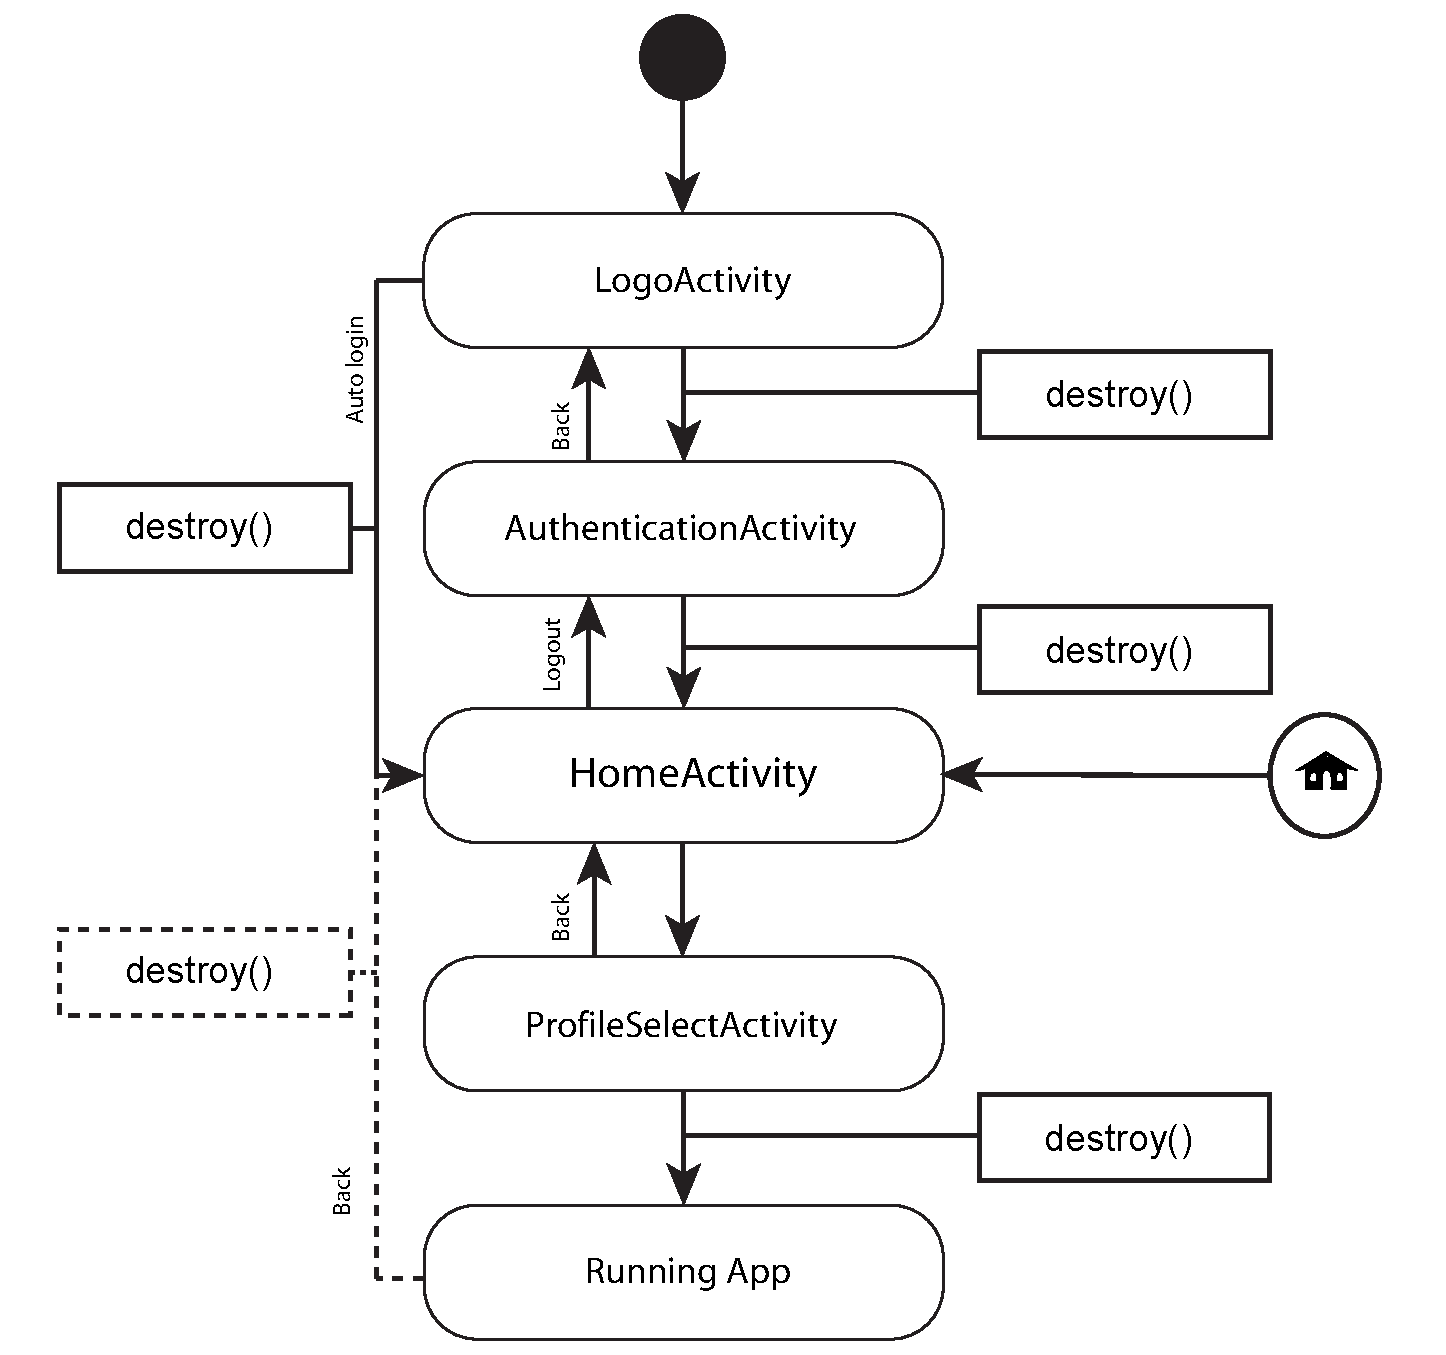
\includegraphics[width=1\textwidth]{gfx/activityDiagram.pdf}
	\caption{Activity diagram of the launcher}
	\label{fig:activity_diagram}
\end{figure}
Figure~\ref{fig:activity_diagram} shows the activity structure of the \giraf[] launcher. Every transition with a \verb+destroy()+ box on it gets the activity starting the transition destroyed. Everytime the user is outside the launcher and hits the home button they will end up in the \activity{HomeActivity}, if the \giraf[] launcher is set to the default launcher.
The dotted line from Running App to \activity{HomeAcitivity} symbolizes that the app it self can handle the back press but if there is not done something to handle this action the default action is to return to the \activity{HomeAcitivity} and destroy the app from the backstack.

When the launcher is started the user is presented with the \activity{LogoActivity} from where they will be redirected to the \activity{AuthenticationActivity} to preform the login. In this process the \activity{LogoActivity} gets destroyed from the backstack.
When the user have pre


\todo{REFACTOR GIRAF COMPONENTS!}